\chapter{Analysis}
\label{chap:analysis}

\section{Alternatives}\label{sec:alternatives}

\xxx{From this point on, the document is a mess.}

Is it worth it?
What will it bring to the table\ldots

Non-virtual versioning file systems\ldots % have already been described on \href{https://en.wikipedia.org/wiki/Versioning_file_system}{Wikipedia}.

In addition, there are several virtual file systems (VFS) with versioning capabilities:

\begin{itemize}
\item There are two user space file systems written using FUSE:
\begin{itemize}
\item \href{https://github.com/FooSoft/vfs}{Simple versioning file system created for Linux with FUSE}, written in Go.
\item \href{https://www.usenix.org/legacy/events/usenix04/tech/freenix/cornell.html}{Wayback: A User-level Versioning File System for Linux}, which was written in Perl for the USENIX 2004 Annual Technical Conference using the old FUSE\@.
\end{itemize}
\item \href{https://osm.hpi.de/vvfs/}{Copy-on-Write Version Support for VFS under Linux} by Stephan Müller and Sven Widmer, implemented as a kernel patch.
\item \href{https://wiki.tcl-lang.org/page/A+versioning+virtual+filesystem}{A versioning virtual filesystem by Steve Huntley}, written with Tcl.
However, this is more of a language demonstration than a practical solution.
\end{itemize}

These products have various limitations, such as being Linux-only or being discontinued.
On the other hand, VFS with encryption is far less prevalent, although there are numerous non-virtual VFS with encryption capabilities, as documented on their \href{https://en.wikipedia.org/wiki/Encrypting_File_System}{Wikipedia page}.
The only example found that closely resembles the desired functionality is \href{https://github.com/rmind/rvault}{rvault}, which focuses on encrypting small files (passwords, keys, and secrets) and makes them available through one-time password authentication.
However, this differs from the intended functionality of this project.

Thus, the primary competition comes from higher-level applications that offer versioning and encryption functionality.
These applications come with their own set of drawbacks, such as the need to constantly run a background program (with access to all files) and limited extensibility for adding other features.
In most cases, incorporating additional features in these applications would not be feasible or practical.

\section{FUSE}\label{sec:fuse-analysis}

Even though There is an option to write kernel drivers\ldots

FUSE (Filesystem in Userspace) is a prominent library for creating a VFS in C++.
It enables developers to implement custom file systems in user space without modifying kernel code.
FUSE provides a comprehensive API for defining file system operations, making it a suitable choice for building a VFS in C++.
Although FUSE was initially designed for Linux, there are variants available for other platforms:

\begin{figure}[ht]
    \centering
    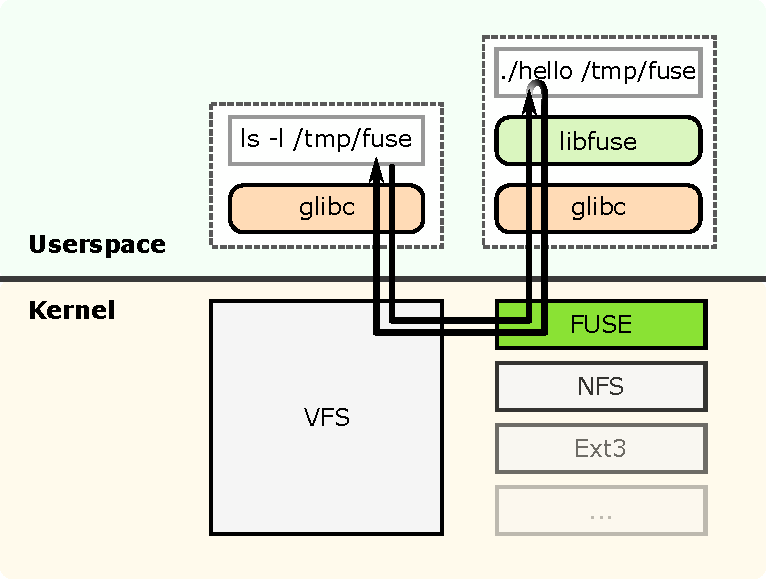
\includegraphics[width=\linewidth]{img/fuse_diagram}
    \caption{FUSE flow-chart diagram}
    \label{fig:fuse-diagram}
\end{figure}

\ldots

\begin{itemize}
\item \textbf{Linux}: \href{https://github.com/libfuse/libfuse}{libfuse} - The reference implementation of FUSE\@.
\item \textbf{macOS}: \href{https://osxfuse.github.io/}{FUSE for macOS} - A macOS port of FUSE\@.
\item \textbf{Windows}: \href{https://github.com/billziss-gh/winfsp}{WinFsp} - A Windows File System Proxy that provides FUSE-compatible functionality.
\end{itemize}

\section{Encryption}\label{sec:encryption-analysis}

\href{https://www.cryptopp.com/}{Crypto++} is a free C++ class library of cryptographic schemes.
It offers a wide range of cryptographic algorithms for encryption, hashing, and authentication.
Crypto++ can be used to implement file-level encryption within the VFS, ensuring data security and privacy.

\subsection{Gtest}\label{subsec:gtest}

\href{https://github.com/google/googletest}{Google Test} (also known as gtest) is a widely-used C++ testing framework developed by Google.

\ldots

\section{Basic idea of creating a VFS}\label{sec:basic-idea-of-creating-a-vfs}

\ldots

\section{Build system and multiplatform challenges}\label{sec:build-system-and-multiplatform-challenges}

Use of CMake, problem with M1 Mac and Windows\ldots even though portable